\documentclass[a4paper]{article}
\usepackage[T1]{fontenc}
\usepackage[english]{babel}
\usepackage{clrscode4e} % Algorithm template from Introduction to Algorithms 4th
\usepackage[left=2cm,right=2cm,top=1cm,bottom=2cm]{geometry} % page settings
\usepackage{amsthm, amsmath, amssymb} % provides many mathematical environments & tools
\usepackage{tikz} % draw pictures
\usepackage{tabularray}
\usepackage[noend]{algorithmic}
\usepackage{tabularx}
\usepackage{algorithm}
\usepackage{arydshln}
\usepackage{forest}
% rotation
\usepackage{adjustbox}
\usepackage{array}
\usepackage{ifthen}
% figure caption
\usepackage{caption}
\usepackage{subfig}
\usepackage{graphicx,wrapfig,lipsum}
% arrays and matrices
\usepackage{nicematrix}
% line change inside cells
\usepackage{makecell}
\usepackage{datetime}
%-----------------------------------------------------------
% Custom commands
%-----------------------------------------------------------
\newenvironment{hashtable}[1][]
  {\begin{tabular}[#1]{
     @{}
     > {\small} r <{\normalsize~\rlap{\fbox{\strut~~}}$~~\rightarrow$~}
     @{} l @{}}}
  {\end{tabular}}

\tikzset{
node of list/.style = {
             draw,
             fill=orange!20,
             minimum height=6mm,
             minimum width=6mm,
             node distance=6mm
   },
link/.style = {
     -stealth,
     shorten >=1pt
     },
array element/.style = {
    draw, fill=white,
    minimum width = 6mm,
    minimum height = 10mm
  }
}

\def\LinkedList#1{%
  \foreach \element in \list {
     \node[node of list, right = of aux, name=ele] {\element};
     \draw[link] (aux) -- (ele);
     \coordinate (aux) at (ele.east);
  }
}

\usetikzlibrary{positioning,matrix, arrows.meta}
\tikzset{box/.style={draw, thick, minimum width=1cm, minimum height=1cm}}

\newcommand{\Mod}[1]{\ (\mathrm{mod}\ #1)}

\newenvironment{solution}
  {\begin{proof}[Solution]}
  {\end{proof}}
\renewcommand{\qedsymbol}{\rule{0.7em}{0.7em}}

\makeatletter
\renewenvironment{proof}[1][\proofname]{%
  \par\pushQED{\qed}\normalfont%
  \topsep6\p@\@plus6\p@\relax
  \trivlist\item[\hskip\labelsep\bfseries#1\@addpunct{.}]%
  \ignorespaces
}{%
  \popQED\endtrivlist\@endpefalse
}
\makeatother
\setlength{\parindent}{0mm}

%-----------------------------------------------------------
% Document
%-----------------------------------------------------------
\begin{document}

\title{Algorithms: Homework 3}
\author{Li-Yuan Wei}
% day-month-year
\newdate{date}{14}{6}{2023}
\date{\displaydate{date}}
\maketitle

\subsection*{Problem 1}
Give an $\mathcal{O}(n^2)$-time algorithm to find the longest monotonically increasing subsequence of $n$ numbers.
\begin{solution}
\end{solution}

\subsection*{Problem 2}
Find an optimal solution to the following activity selection problem:

\begin{figure}[H]
\centering
\begin{minipage}{5cm}
\centering
$\begin{NiceArray}{*{10}{c}}[first-row, first-col, hvlines]
\CodeBefore
\Body
i  & 1 & 2 & 3 & 4 & 5 & 6 & 7 & 8 & 9 & 10\\
s_i & 1 & 3 & 2 & 3 & 5 & 8 & 7 & 10 & 5 & 11\\
f_i & 3 & 4 & 5 & 6 & 8 & 9 & 11 & 12 & 14 & 15
\end{NiceArray}$
\end{minipage}
\end{figure}

\begin{solution}
The optimal solution is to chose the following events: <1, 2, 5, 6, 8>.
\end{solution}


\subsection*{Problem 3}
Not just any greedy approach to the activity-selection problem produces a maximum-size set of mutually compatible activities. (a) Give an example to show that the approach of selecting the activity of least duration from those that are compatible with previously selected activities does not work. (b) Do the same for the approaches of always selecting the compatible activity that overlaps with the fewest other remaining activities by selecting the compatible remaining activity with the earliest start time.

\begin{solution}
\end{solution}

\subsection*{Problem 4}
Give a dynamic-programming solution to the 0-1 knapsack problem that runs in $\mathcal{O}(nW)$ time, where $n$ is number of items and $W$ is the maximum weight of items that the thief can put in his knapsack. Note that $W$, as well as all the weights of the involved items are integers.
\begin{solution}
\end{solution}

\subsection*{Problem 5}
Assume there are only 7 characters A, B, C, D, E, F and G in a document, with occurrences of 6, 4, 8, 3, 2, 1 and 5, respectively. Please calculate the total number of bits of this document after applying the Huffman coding.
\begin{solution}
C: 8, 0
A: 6, 10
G: 5,
B: 4,
D: 3,
E: 2,
F: 1
\begin{figure}[H]
\centering
\begin{minipage}{5cm}
\centering
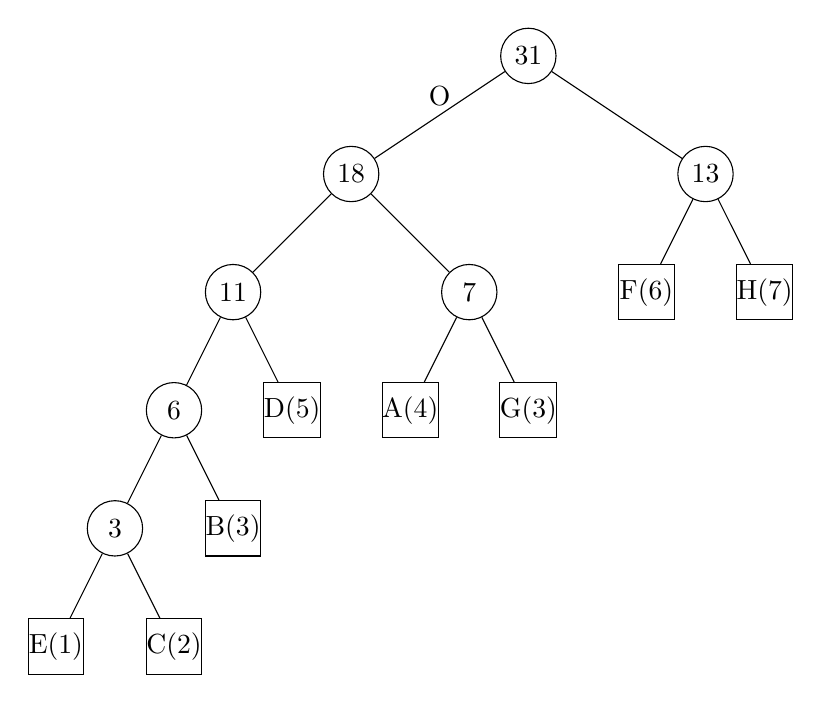
\begin{tikzpicture}[iv/.style={draw,circle,minimum size=20pt,inner
sep=0pt,text=black},ev/.style={draw,rectangle,minimum
size=20pt,inner sep=0pt,text=black}]
\node[iv]{31}
  child {node[iv]{18}
         child {node[iv]{11}
                child {node[iv]{6}
                       child {node[iv]{3}
                              child {node[ev]{E(1)}}
                              child {node[ev]{C(2)}}
                             }
                       child {node[ev]{B(3)}}
                      }
                child {node[ev]{D(5)}}
                }
         child [missing]
         child {node[iv]{7}
         child {node[ev]{A(4)}}
         child {node[ev]{G(3)}}
               }
        edge from parent node[above]{O}
        }
  child [missing]
  child [missing]
  child {node[iv]{13}
         child {node[ev]{F(6)}}
         child {node[ev]{H(7)}}
        };
\end{tikzpicture}
\caption{Huffman code tree}
\end{minipage}
\end{figure}
\end{solution}

\subsection*{Problem 6}
Represent the graph on the right by adjacency-matrix and adjacency-list.
\begin{solution}
\begin{figure}[H]
\centering
\begin{minipage}{5cm}
\centering
$\begin{NiceArray}{*{5}{c}}[first-row, first-col, hvlines, name=amatrix]
  & 1 & 2 & 3 & 4 & 5 \\
1 & 0 & 1 & 0 & 1 & 0 \\
2 & 1 & 0 & 1 & 1 & 0 \\
3 & 0 & 1 & 0 & 0 & 1 \\
4 & 1 & 1 & 0 & 0 & 1 \\
5 & 0 & 0 & 1 & 1 & 0 \\
\end{NiceArray}$
\caption{adjacency-matrix}
\end{minipage}
\qquad
\begin{minipage}{5cm}
\centering
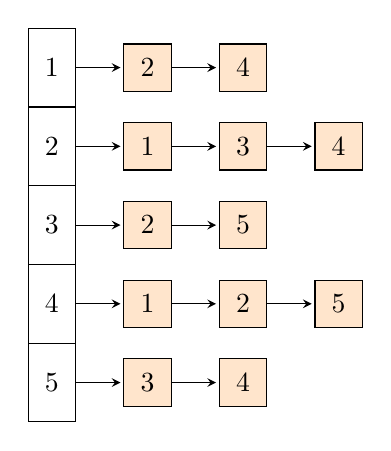
\begin{tikzpicture}
  \foreach \index/\list in {1/{2, 4}, 2/{1, 3, 4}, 3/{2, 5}, 4/{1, 2, 5}, 5/{3, 4}} {
   \node[array element] (aux) at (0,-\index) {\index};
   \LinkedList{\list}
}
\end{tikzpicture}
\caption{adjacency-list}
\end{minipage}
\end{figure}
\end{solution}

\subsection*{Problem 7}
Show the $d$ and $\pi$ values that result from running the breadth-first search on the same graph using vertex 3 as the source.
\begin{solution}
\end{solution}

\subsection*{Problem 8}
(a) Show how depth-first search works on the graph at the bottom. Assume that the for loop of lines 5—7 of the DFS procedure considers the vertices in alphabetical order, and assume that each adjacency list is ordered alphabetically. Show the discovery and finishing time for each vertex, and show the classification of each edge. (b) According to (a), show the corresponding topological sort of this graph.
\begin{solution}
\end{solution}

\subsection*{Problem 9}
Find the strongest components of the following graph:
\begin{solution}
\end{solution}

\subsection*{Problem 10}
Find the minimal spanning tree of the following graph, using (a) Kruskal’s algorithm, (b) Prim’s algorithm (using q as the starting vertex). Please give the selected edge in order during the spanning tree construction process
\begin{solution}
\end{solution}
\end{document}


